\chapter{Analyse exploratoire}

Les données brutes étant collectées, l’objectif est désormais de les analyser pour les comprendre et préparer le feature engineering avant de rechercher un modèle.

Dans cette section, nous allons :

\begin{itemize}
\item Faire le bilan des observations et des variables disponibles ;
\item Vérifier leur type ;
\item Vérifier si des valeurs sont manquantes ou aberrantes ;
\item Etudier leur relations potentielles.
\end{itemize}

\section{Variables disponibles}
\label{subsec:var_dispo}

Le jeu de données collecté comprend 86 variables pour 105 170 observations à une résolution temporelle de 30 minutes entre le 31 décembre 2019 (1er janvier 2020 heure française) et le 30 décembre 2025 (date de fin de service du satellite ayant collecté les données de nébulosité).

Aucune observation n’est manquante : le jeu de données comprend bien une et une seule observation toutes les 30 minutes du début à la fin de la collecte.

Par ailleurs, toutes les variables sont de type numérique (float64) à l’exception de la variable temporelle \textit{datetime\_utc} utilisée comme index (DatetimeIndex).

Enfin, il n’y a ni valeur manquante, ni doublons.

On dispose de 6 variables concernant l’ensemble de la région :

\begin{itemize}
\item \textbf{consommation} : consommation électrique totale du périmètre considéré sur l'intervalle de temps donné.
\item \textbf{datetime\_utc} : horodatage en temps universel coordonné (UTC) correspondant à l'instant d'agrégation des données (résolution 30 minutes).
\item \textbf{solaire} : production électrique issue des installations photovoltaïques sur le périmètre considéré.
\item \textbf{target} : variabilité absolue du taux de charge de la production solaire à t + 30 minutes (notre variable cible).
\item \textbf{tco\_solaire} : taux de couverture de la production solaire.
\item \textbf{tch\_solaire} : taux de charge de la production solaire.
\end{itemize}

Outre ces six variables à l’échelle régionale, on dispose de 16 variables pour les cinq points d'intérêts de la production photovoltaïque régionale (ce qui représente 16 x 5 = 80 colonnes) :

\begin{itemize}
\item \textbf{altitude} : altitude solaire (en degrés), représentant l'élévation du soleil au-dessus de l'horizon (valeurs négatives durant la nuit).
\item \textbf{azimuth} : azimut solaire (en degrés), indiquant la direction du soleil par rapport au nord (0–360° selon la convention).
\item \textbf{bhi} \textit{(Beam Horizontal Irradiance)} : composante directe du rayonnement solaire projetée sur le plan horizontal (Wh/m²).
\item \textbf{bni} \textit{(Beam Normal Irradiance)} : irradiance directe normale, reçue sur un plan perpendiculaire aux rayons solaires (Wh/m²).
\item \textbf{clear\_sky\_bhi} : composante directe horizontale en conditions de ciel clair (Wh/m²).
\item \textbf{clear\_sky\_bni} : irradiance directe normale en conditions de ciel clair (Wh/m²).
\item \textbf{clear\_sky\_dhi} : composante diffuse horizontale en conditions de ciel clair (Wh/m²).
\item \textbf{clear\_sky\_ghi} : irradiance globale horizontale en conditions de ciel clair, utilisée comme référence théorique sans nuages (Wh/m²).
\item \textbf{dhi} \textit{(Diffuse Horizontal Irradiance)} : composante diffuse du rayonnement solaire reçue sur un plan horizontal (Wh/m²).
\item \textbf{ghi} \textit{(Global Horizontal Irradiance)} : irradiance globale reçue sur un plan horizontal (composantes directe et diffuse) exprimée en Wh/m².
\item \textbf{humidite} : humidité de l'air (généralement humidité relative en %, ou humidité spécifique selon la source).
\item \textbf{nebulosite} \textit{(souvent cloud\_AMT)} : nébulosité ou fraction de couverture nuageuse (exprimée selon les produits en fraction, pourcentage ou indice adimensionnel).
\item \textbf{reliability} : fiabilité des données CAMS (\textit{bhi}, \textit{bni}, \textit{clear\_sky\_bhi}, \textit{clear\_sky\_bni}, \textit{clear\_sky\_dhi}, \textit{clear\_sky\_ghi}, \textit{dhi}, \textit{ghi}, \textit{toa}).
\item \textbf{temperature} \textit{(souvent T2M)} : température de l'air à 2 mètres du sol (en °C ou en K selon la source ; une vérification des unités est nécessaire).
\item \textbf{toa} \textit{(Top Of Atmosphere)} : rayonnement solaire incident au sommet de l'atmosphère (Wh/m²), utilisé pour le contrôle de cohérence et la normalisation des séries.
\item \textbf{vitesse\_vent} \textit{(souvent V2M)} : vitesse du vent mesurée à 2 mètres du sol (m/s).
\end{itemize}

\begin{figure}[htbp]
    \centering
    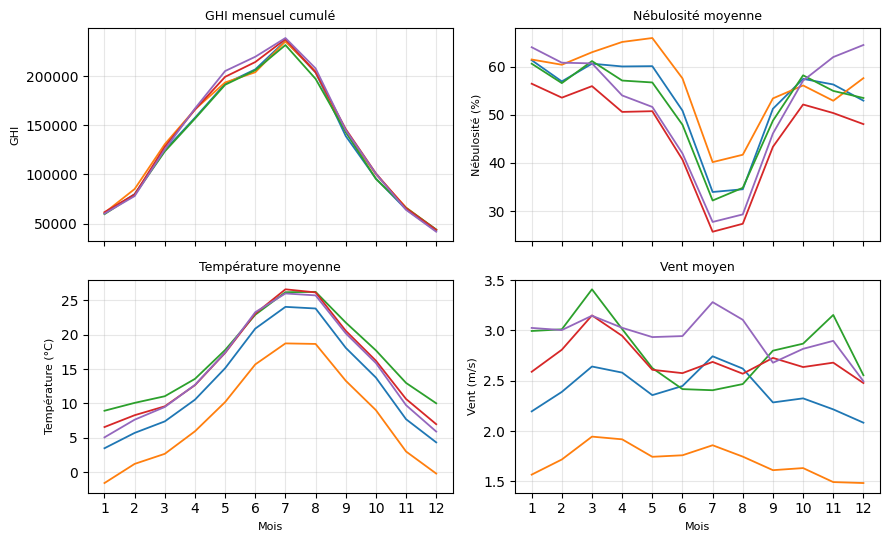
\includegraphics[width=0.9\textwidth]{img/ex_meteo.png}
    \caption{Comparaisons de variables prises aux cinq points significatifs.}
    \label{fig:comparaisons_5pts}
\end{figure}

On remarque toutefois qu’à quelques exceptions près (dhi, nébulosité et vitesse du vent), chacune de ces variables présente une forte colinéarité entre elles, ce que confirme une analyse du VIF (Variance Inflation Factor).

\textbf{Plus de détails} sur les tests statistiques sur les variables communales sont disponibles dans notebooks/03\_Analyse/03\_analyse\_01\_exploration\_preliminaire.ipynb.

Afin de faciliter l’analyse de ces variables communales, on décide de les remplacer par leur somme pondérée par la contribution des communes correspondantes à la production d’énergie solaire régionale.

Exemple pour la variable GHI :

\begin{equation}
GHI_{region} = \sum_{i=1}^{5}p_{i}.GHI_{i}
\end{equation}

Avec :

\begin{itemize}
\item $GHI_{region}$ la somme pondérée obtenue pour remplacer les cinq variables GHI communales ;
\item $i$ une commune parmis les cinq communes d’intérêt ;
\item $GHI_{i}$ la valeur de la variable GHI dans la commune i ;
\item $p_{i}$ le poid correspondant à la part de la contribution à la production photovoltaïque de la région par la commune i.
\end{itemize}

\section{Distribution des variables}

Afin d’explorer la distribution des variables météorologiques régionales construites par agrégation pondérée, une analyse exploratoire est réalisée à l’aide de boxplots.

Exemple pour les variables mesurées au niveau communale :

\begin{figure}[htbp]
    \centering
    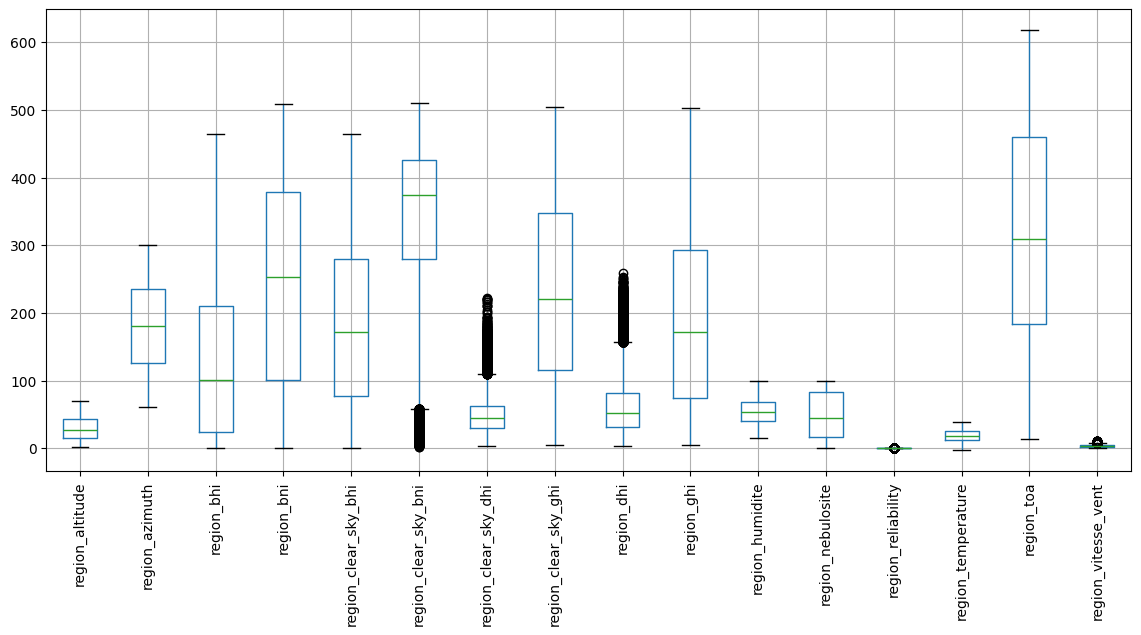
\includegraphics[width=0.9\textwidth]{img/distrib_5pts.png}
    \caption{Distributions des variables mesurées au niveau communal puis aggrégées.}
    \label{fig:distrib_5pts}
\end{figure}

Les distributions des variables sont diverses : les échelles de valeurs diffèrent parfois de deux ordres de grandeur. Une normalisation des données pourra être pertinente pour certains algorithmes de modélisation.

Les variables \textit{region\_clear\_sky\_bhi}, \textit{region\_clear\_sky\_dhi} et \textit{region\_dhi} présentent des valeurs extrêmes, mais celles-ci ne paraissent pas aberrantes.

Il en va de même pour les variables collectées directement au niveau régional.

L’étude de la variance des variables permet de constater que la variable \textit{reliability} (qui concerne la fiabilité des données atmosphériques) a une variance inférieure à 0.01, ce qui la rend peu exploitable en pratique : elle sera mise de côté lors de l’étape de feature engineering.

\section{Exploration de la variable cible}

Dans cette section, nous allons explorer la manière dont se comporte notre variable cible au cours d’une journée, d’une année et par rapport aux variables TCH solaire et GHI. D’autres études ont été menées dans le notebook correspondant (cité en fin de section).

On s’intéresse tout d’abord à l’évolution moyenne de la variable cible et de la production d’énergie solaire (tch solaire) au cours d’une journée, en excluant la nuit où le soleil est couché :

\begin{figure}[htbp]
    \centering
    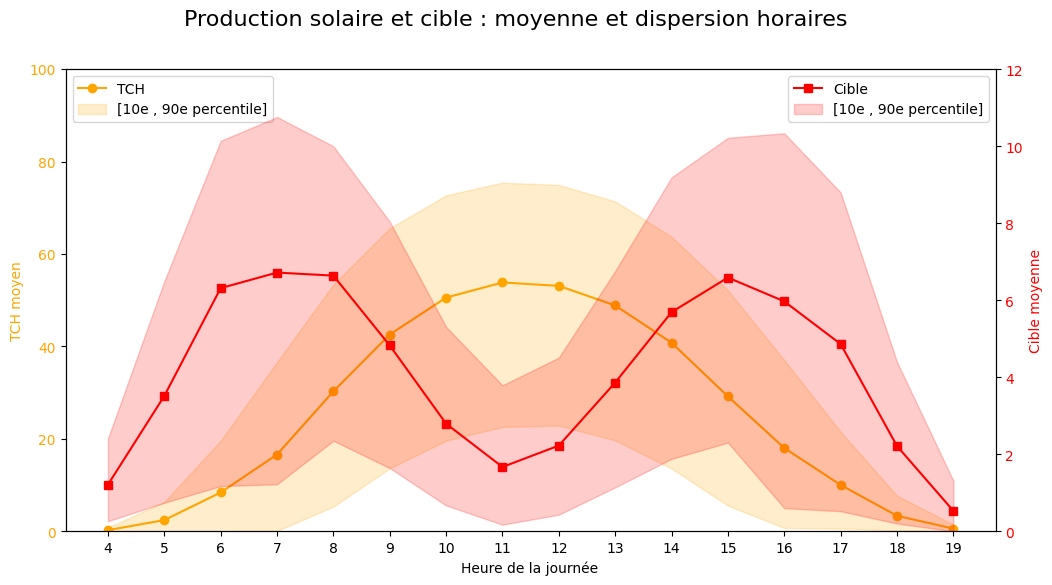
\includegraphics[width=0.9\textwidth]{img/cible_tch_jour.png}
    \caption{Comparaison du TCH et de sa variabilité au cours de la journée : moyenne et dispersion.}
    \label{fig:cible_tch_jour}
\end{figure}

\begin{itemize}
\item La production solaire est \textbf{faible et relativement instable en proportion} en début et fin de journée (variabilité élevée).
\item Elle est \textbf{maximale et la plus régulière autour de midi}, caractérisée par une \textbf{forte moyenne et une faible variabilité}.
\end{itemize}

Cette analyse permet d'identifier les \textbf{heures les plus stables} (milieu de journée) et celles où la \textbf{variabilité est la plus forte} (matin et après-midi).

\clearpage

Si on s’intéresse maintenant aux statistiques saisonnières, on constate :

\begin{figure}[htbp]
    \centering
    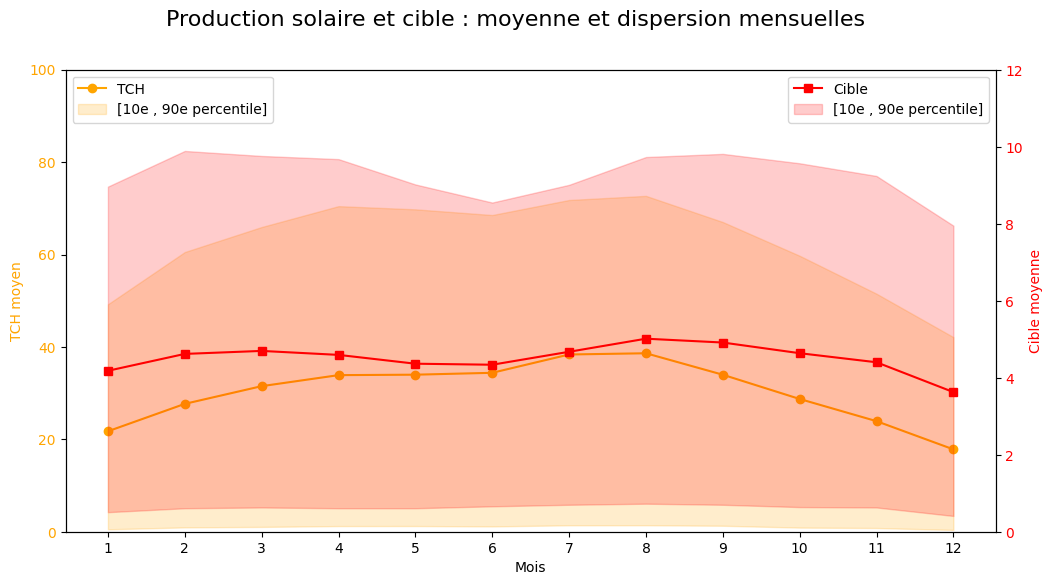
\includegraphics[width=0.7\textwidth]{img/cible_tch_mois.png}
    \caption{Comparaison du TCH et de sa variabilité au cours de l'année : moyenne et dispersion.}
    \label{fig:cible_tch_mois}
\end{figure}

\begin{itemize}
\item Que la \textit{cible} est plus \textbf{faible} et plus \textbf\textbf en \textbf{mai et juin} ainsi qu'en \textbf{décembre et en janvier} ;
\item Qu’en automne et en hiver, la production est \textbf{plus régulière relativement à son niveau moyen}.
\end{itemize}

Enfin on peut également analyser la variation de la variable cible et du tch solaire en fonction de la variable GHI qui témoigne de l’irradiance solaire reçue au niveau des panneaux solaires :

\begin{figure}[htbp]
    \centering
    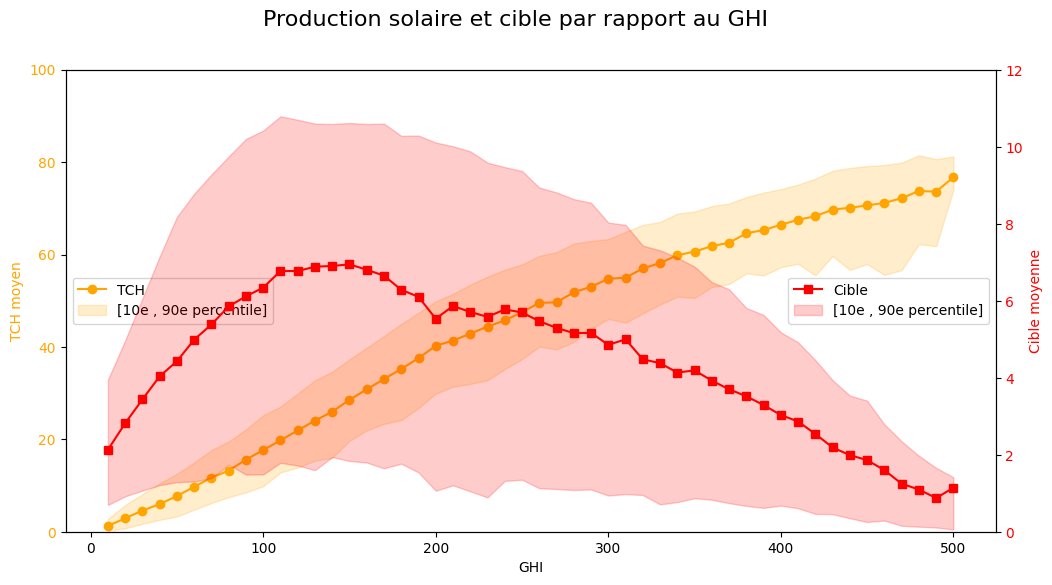
\includegraphics[width=0.7\textwidth]{img/cible_tch_ghi.png}
    \caption{TCH et variabilité du TCH en fonction du GHI : moyenne et dispersion.}
    \label{fig:cible_tch_ghi}
\end{figure}

\begin{itemize}
\item La moyenne de TCH augmente régulièrement avec le GHI, ce qui traduit une relation cohérente entre irradiance et production.
\item La variabilité de la production solaire est faible aux faibles GHI (peu de production au lever et coucher du jour), atteint un maximum vers GHI = 150, ce indique une variabilité relative importante pour une production moyenne faible. Au-delà de cette valeur du GHI, la variabilité de la production solaire diminue progressivement lorsque le GHI augmente : la production devient alors plus stable proportionnellement à sa moyenne.
\end{itemize}

\textbf{Plus de détails} sur les distributions des variables et leurs relation entre elles sont disponibles dans notebooks/03\_Analyse/03\_analyse\_02\_exploration\_detaillee.ipynb.
